\chapter{Neural networks}\label{ch:neural-networks}


\textit{Artificial neural networks} (ANNs), or just neural networks, are a class of mathematical models used for various tasks, including data classification, self-driving, chatbots, sentiment analysis, time series prediction, computer vision, art generation, and many more.
As the name suggests, ANNs are a set of artificial \textit{neurons} specially arranged into so-called layers.
Neural networks are somewhat inspired by biological neural nets;
hence we will now briefly examine them.~\cite{ann-basics}

The brain consists of many neurons (figure~\ref{fig:bio-neuron}) consisting of dendrites, a cell body, and an axon.
Dendrites are branched connections of a neuron that received propagate the electrochemical stimulation received from other neurons and send them to the cell body, where the signals are summed up, and once the triggering threshold is reached, the signal propagates through the axon.
The last part of a neuron is the axon, the long connection leading from a neuron that transmits a signal to different neurons, muscles, or glands.
Neurons can communicate with other neurons' dendrites and other body parts via these connections, so-called synapses, and pass on their electrochemical potential.
A depiction of the triggering threshold and voltage output is illustrated in figure~\ref{fig:bio-neuron-activation}.~\cite{ann-basics}

\begin{figure}
    \centering
    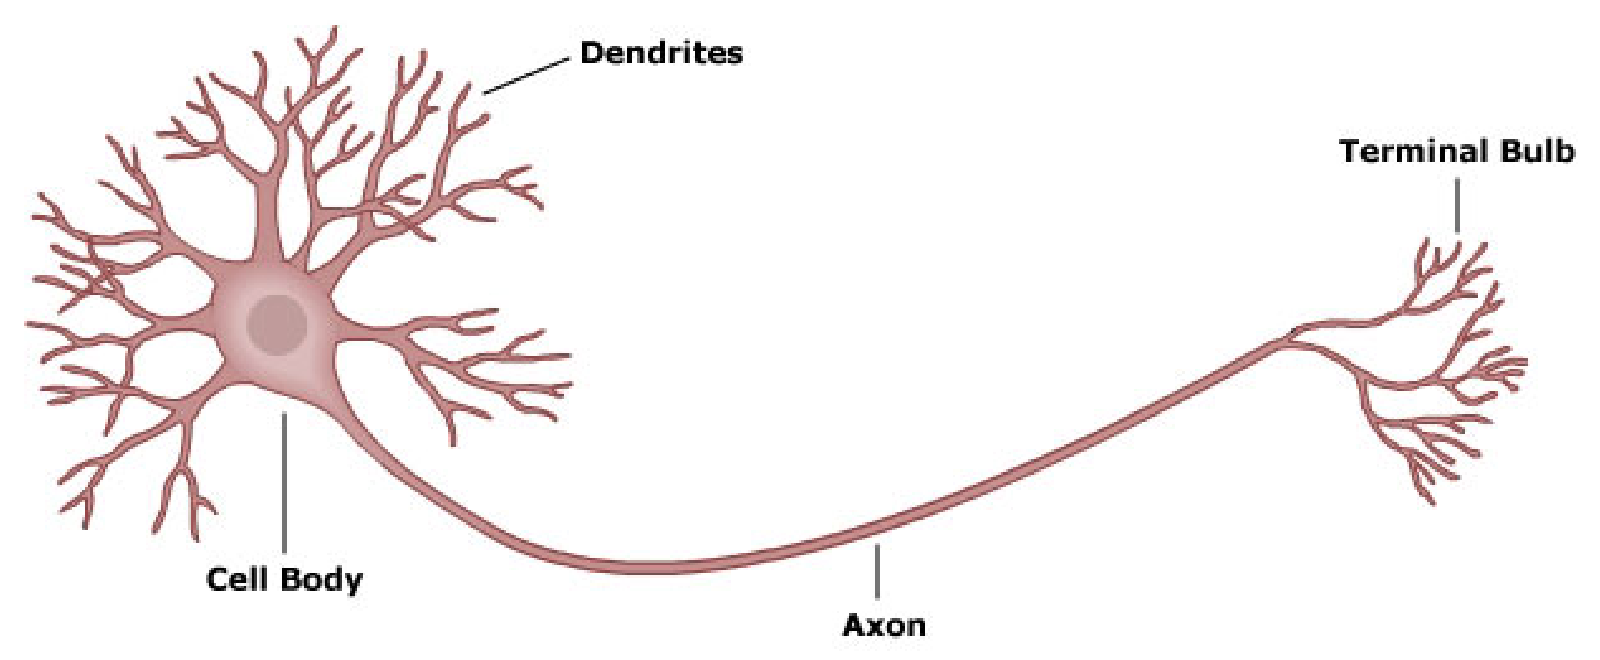
\includegraphics[width=0.74\textwidth]{assets/biological-neuron}
    \caption{~A typical biological neuron~\cite{ann-basics}}\label{fig:bio-neuron}
\end{figure}


\begin{figure}
    \centering
    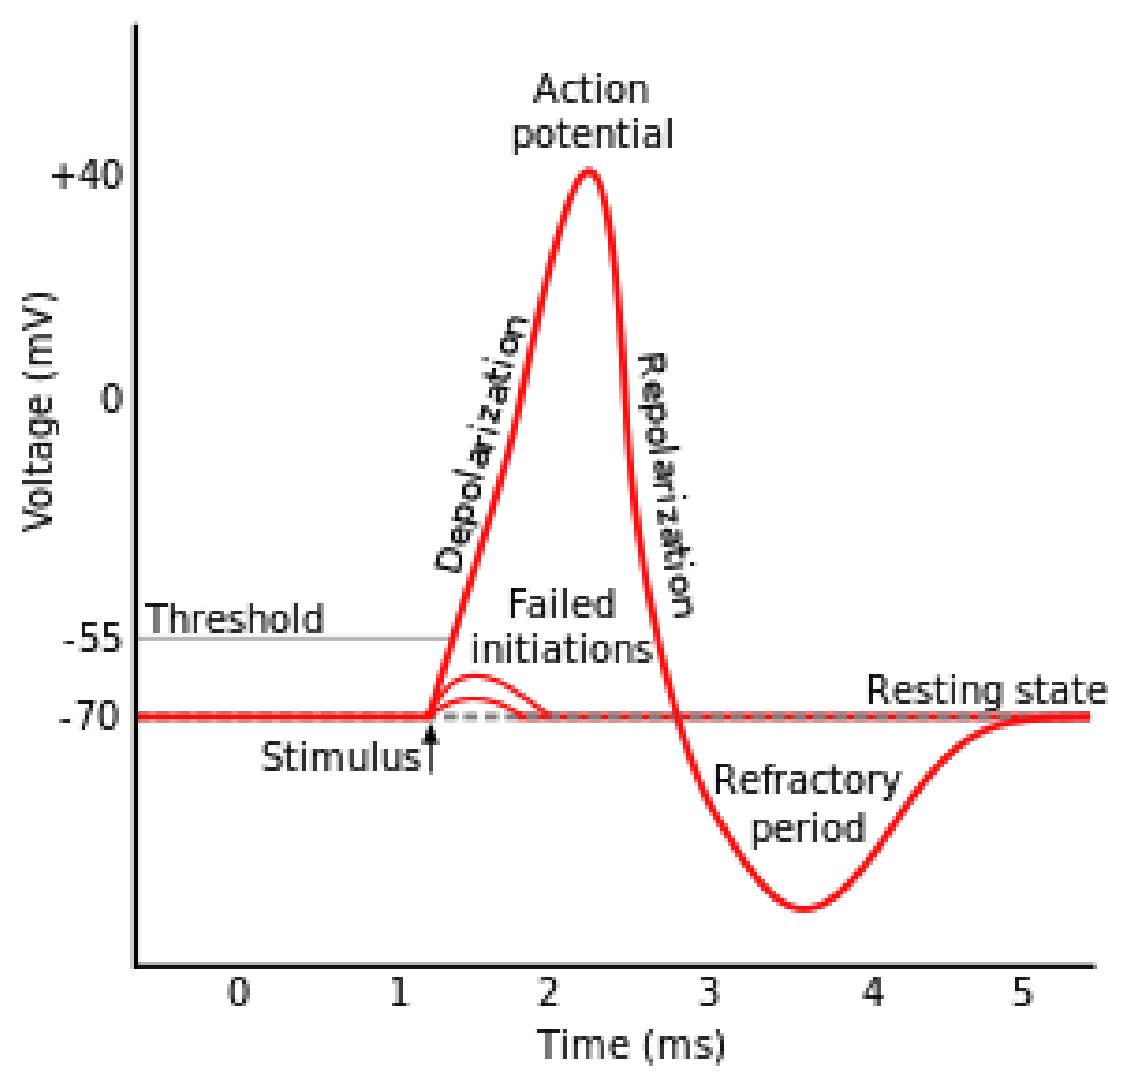
\includegraphics[width=0.4\textwidth]{assets/biological-neuron-activation}
    \caption{~Representation of action potentials and the triggering threshold needed to propagate a signal~\cite{ann-basics}}\label{fig:bio-neuron-activation}
\end{figure}


\section{Neurons}\label{sec:neurons}

Now let's look at a mathematical model of an \textit{artificial neuron}.
This model contains three input nodes: $X_1$, $X_2$, and $X_3$, that channel their output values multiplied by their respective weights $w_{11}$, $w_{12}$, and $w_{13}$, into the neuron ``body.''
We denote $n$ dendrites in the input layer nodes as $x_1$, $x_2$, $x_3$, \ldots, $x_n$ and their corresponding $m$ weights as $w_{11}$, $w_{12}$, \ldots, $w_{nm}$, where $w_{ij}$ refers to the weight taking $x_j$ to the node $i$.
The body of an artificial neuron works simply by summing input values multiplied by the connection \textit{weights} along with the neuron \textit{``bias''} term $b$ (this can be thought of as neuron resting-state potential) and passes the summed value to an $activation function$.
The activation function is usually one of the nonlinear transfer functions described later.
This value is either fed into the following layer of neurons or outputted out of the model.
A simplified model of the artificial neuron can be seen in figure~\ref{fig:artificial-neuron}.~\cite{ann-basics}


\begin{figure}
    \centering
    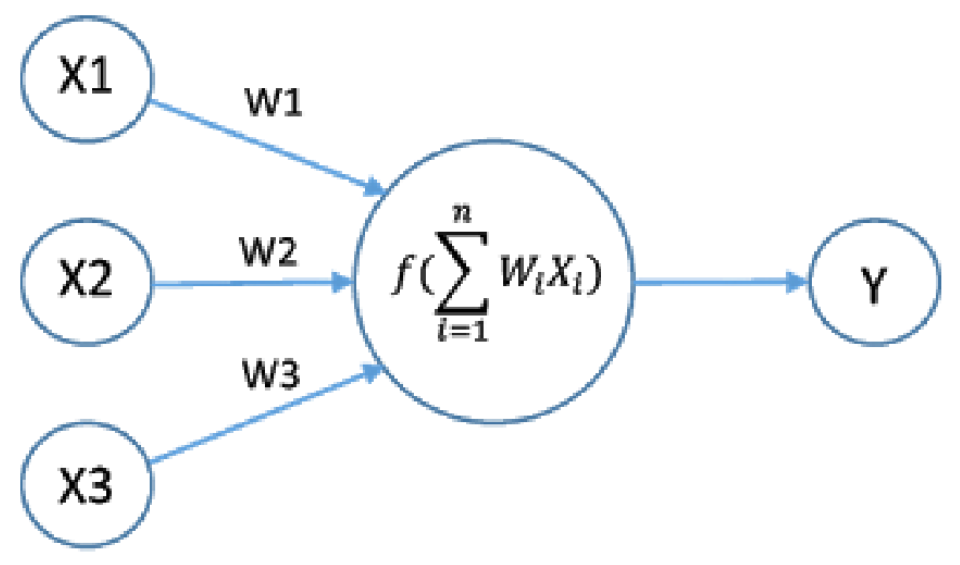
\includegraphics[width=0.4\textwidth]{assets/artificial-neuron}
    \caption{~A mathematical depiction of an artificial neuron~\cite{ann-basics}}\label{fig:artificial-neuron}
\end{figure}

A mathematical formula for neuron internal potential is following: \[ y = (w_{11}, w_{12}, \ldots, w_{1n}) \times
\begin{blockarray}{c}
    \begin{block}{[c]}
        x_{11} \\
        x_{12} \\
        x_{13} \\
        \vdots \\
        x_{1n} \\
    \end{block}%
\end{blockarray}%
= w_{11}x_1 + w_{12}x_2 + \ldots + w_{1n}x_n + b = \textbf{w} \times \textbf{x} + b
\]

Later we apply an \textit{activation function} (figure~\ref{fig:activation-functions}) $\sigma$ to the node’s \textit{internal potential}, $\sigma (y)$ is the output of a single neuron.
The activation function corresponds to the activation state of a node.
As mentioned earlier, a voltage potential must build up enough signal in the cell body to send a signal down the axon.
The activation function simulates this biological effect in a neural network for the node and output signal.
Overall, this is how we model a single neuron.
A \textit{neural network} is a collection of single neurons arranged into layers.
Therefore, by understanding how a single neuron works, we can better grasp how a neural network functions.~\cite{ann-basics}


\section{Activation functions}\label{sec:activation-functions}

The \textit{activation function}, also known as the \textit{transfer function}, corresponds to the activation state of a neuron.
It simulates the biological effect of overcoming a voltage potential to propagate to an axon.
This function manipulates internal potential (pre-state) and transforms it into the output coming from a node.
Mathematically, the transfer function $\sigma (r)$ has to be differentiable (to allow backpropagation), increasing, and has to have horizontal asymptotes.
$r$ corresponds to a pre-state for which the activation function generates an output.
A couple of typical functions for $\sigma (r)$ will be discussed.~\cite{ann-basics}

These are the formulas for the most common functions:

\begin{align*}
    \sigma (r) &= arctan(r) = tan^{-1}(r), \\[4pt]
    \sigma (r) &= sigmoid(r) = \frac{1}{1 + e^{-r}}, \\[4pt]
    \sigma (r) &= \frac{e^{2r} - 1}{e^{2r} + 1}, \\[4pt]
    \sigma (r) &= reLU(r) = max(0, r)
\end{align*}

You can see these four activation functions plotted in a graph in figure~\ref{fig:activation-functions}.

\begin{figure}
    \centering
    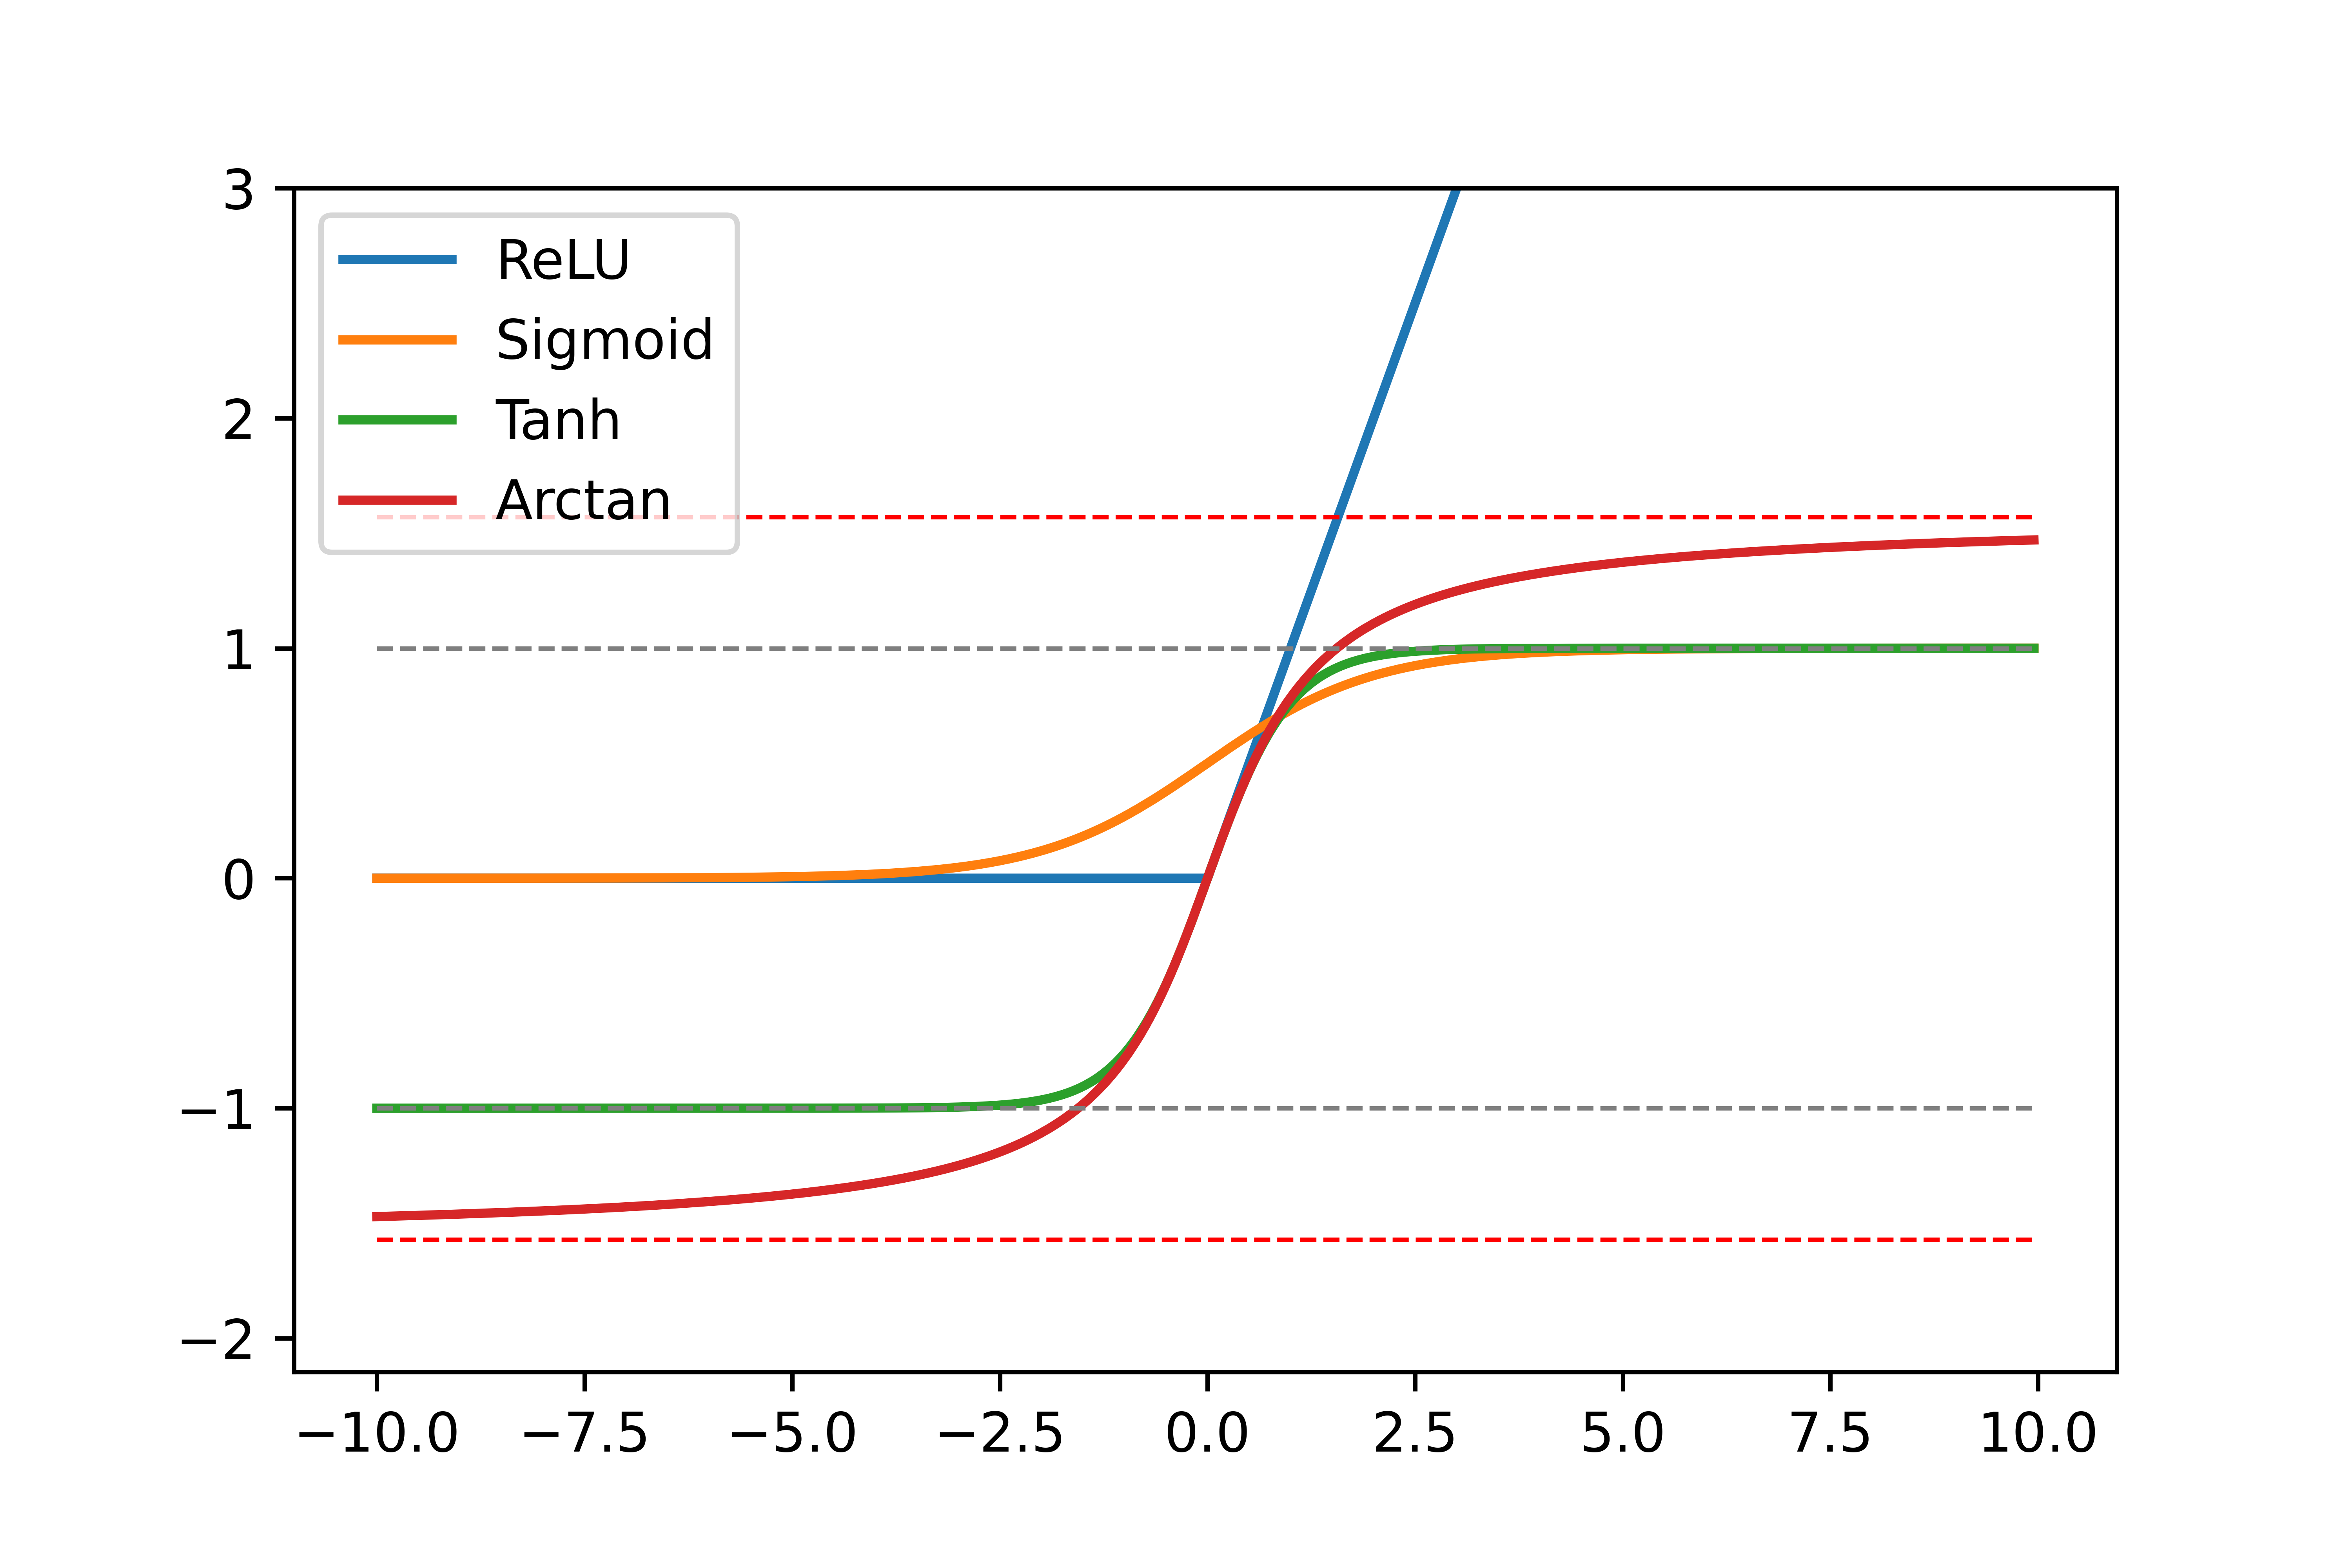
\includegraphics[width=0.7\textwidth]{assets/activation-functions}
    \caption{~Commonly used activation functions}\label{fig:activation-functions}
\end{figure}


\section{Network architecture}\label{sec:network-architecture}

A neural network consists of a sequence of \textit{layers}.
The first layer is called the \textit{input layer}, and the number of neurons (or nodes) in the input layer is derived from the \textit{dimensionality} of the input: $x_i \in \mathbb{R}^n$, the layer has $n$ nodes.
The final layer is called the output layer, and the number of neurons in the output layer is derived from the dimensionality of the output: $y_j \in \mathbb{R}^m$, the layer has $m$ nodes.
In Figure~\ref{fig:ann-architecture}, $x_i \in \mathbb{R}^3$ and $y_j \in \mathbb{R}^1$ so, there are three neurons in the input layer and one neuron in the output layer.
In between the two layers mentioned before are a number of the hidden layers, each containing some number of k neurons.
We define the neural network's \textit{architecture} by the number of nodes in each layer.
For example, figure~\ref{fig:ann-architecture} depicts a neural network with three nodes in the input layer, four nodes in the first hidden layer, four nodes in the second hidden layer, and one node in the output layer.
This network could be described as a 3-4-4-1 neural network.~\cite{ann-basics}


\begin{figure}
    \centering
    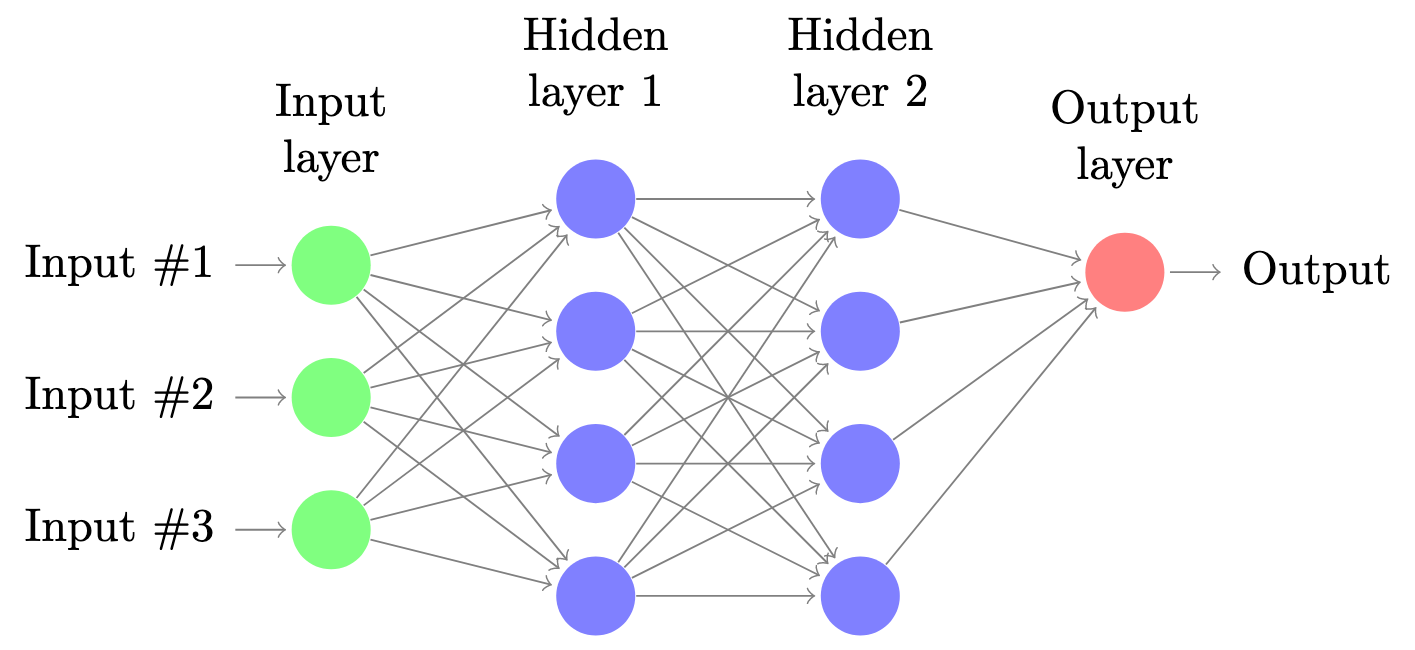
\includegraphics[width=\textwidth]{assets/ann-architecture}
    \caption{~A 3-4-4-1 neural network~\cite{ann-basics}}\label{fig:ann-architecture}
\end{figure}


\section{Training and application of ANNs}\label{sec:training-and-application-of-anns}

A neural network is a model that, when trained, \textit{recognizes patterns} in data sets.
Once a neural net is \textit{trained}, given enough simulation data to recognize the patterns, it can predict outputs in future data.
We can think of training a neural network as \textit{estimating a function} between a given domain and range.
Once trained, any data within the domain we provide can be mapped to the range of the function.
A simple example of a neural network in action is data \textit{classification}.
We are given a data set containing six characteristics of 200 wines (the input would be a $6 \times 200$ matrix) and knowing the properties of 5 different types of wine.
We can train the neural network on 50 different wines, and then the generated function will be able to classify the other 150 wines into the five types of wine (the output would be a $5 \times 200$ matrix).
ANNs can be a powerful tool for \textit{analyzing}, \textit{predicting}, or \textit{generating} data.~\cite{ann-basics}

There are two types of learning: \textit{supervised} learning and \textit{unsupervised} learning.
Supervised learning is when the output or target values are known.
That was the case in the beforementioned example about the wine classification.
In classifying wine into the five types, we knew the correct wine types for the 200 bottles when used as a learning dataset.
Contrary to that, unsupervised learning does not ``know'' the outputs or target values.
The learning process finds \textit{patterns} within the data in order to output values.
Unsupervised learning is used in many complex systems, including data processing, modeling, and classification.
The goal of the training process is to find weight and bias values that produce the most accurate function approximation.
That is easier said than done as there are many caveats when using and training neural networks, like choosing unsuitable network architecture.~\cite{ann-basics}


\section{Feed-Forward Neural Networks}\label{sec:feed-forward-neural-networks}

A \textit{feed-forward} neural network is one of the most straightforward ANN architectures.
It is a part of supervised learning and creates a mapping $\mathbb{R}^n \to \mathbb{R}^m$.
The mapping consists of an initial signal $x$, pre-states $P_j$, activation function $\sigma (r)$, and states $S_j$.
In order to compute the neural network's final output, we have to calculate all these states for each layer.
We start at the input layer and continue forward towards the output layer because each layer depends on the previous one.~\cite{ann-basics}

These are the formulas for calculating pre-states $P_j$ and states $S_j$:

\[
    P_i = W_i S_{i-1} + b_i, S_i = \sigma (P_i)
\]


\section{Backpropagation}\label{sec:backpropagation}

The goal of a neural network is to approximate a function between a given range and domain.
Our aim is to build the function so that the determined outputs equal the given target values, $F (x_i) = \hat y_i$, where $F$ is the function created by ANN, $x_i$ the inputs, and $\hat y_i$ the target values.
The typical to go about this is to create a \textit{loss function} that computes the error between our prediction $\hat y_i$ and the actual output $y_i$.
We then find the values of parameters that minimize it.
The loss function depends on what type of problem we are solving.
\textbf{Mean Squared Error} is mainly used for regression and \textbf{Categorical Cross-Entropy} is most commonly used for classification.~\cite{ann-basics}
Since we know the targets $y_i$ and the outputs $\hat y_i = F (x_i)$ (as we just described earlier), our error functions will be the following:

Mean Squared Error: \[ L=(y_i - \hat y_i)^2 \]

Categorical Cross-Entropy (given M classes): \[ L=\sum_{i=1}^{M} y_i \log \hat y_i \]

The loss function is dependent on the weight matrices $W_i$ and the bias vectors $b_i$ for each layer of the neural network.
In order to decrease the error of the neural net, we will use the \textit{gradient} of the error function.
We calculate the \textit{derivative} of the loss function, compute the \textit{direction of the gradient} and change the weights and biases to move in the \textit{opposite} direction of the gradient.
Moving in the direction of the gradient achieves the fastest ascend, so moving in the direction opposite to the gradient results in the fastest descent.~\cite{ann-basics}
Unsurprisingly this method is called \textit{gradient descent}, where the parameter $u$ (the actual parameters of the function are the weights $W_i$ and biases $b_i$) is updated by:
\[ u_{new} = u_{old} - \alpha \frac{dL}{du} \]

Where α is the learning rate, controlling how big the leaps are taken when updating the weights and biases to reduce error.
\textit{``Generally, a large learning rate allows the model to learn faster, at the cost of arriving on a sub-optimal final set of weights.
A smaller learning rate may allow the model to learn a more optimal or even globally optimal set of weights but may take significantly longer to train.''}~\cite{learning-rate}
We use backpropagation in order to determine the term $\frac{dL}{du}$.
While there are other techniques (like genetic algorithms), \textit{backpropagation} of error is an efficient way of computing the change of the error in a network.
For backpropagation, we first run a  forward pass through the network to determine each node's state conditions.
We determine the partial derivatives through the network to get each node's error term $\Delta^l_m$ when going backward.~\cite{ann-basics}
Following is the formula to update the weight $W^l_{mn}$, which connects node $n$ in layer $l - 1$ to node $m$ in layer $l$:

\[
        \mathit{new}\, W^l_{mn} = W^l_{mn} + \varepsilon \frac{dL}{dW} = W^l_{mn} + \varepsilon \Delta^l_m S^{l-1}_n
\]

$\Delta^l_m$ here means the error term that measures how much node $m$ in layer $l$ was responsible for overall errors in our output, and $S^{l-1}_n$ is the state of node $n$ in layer $l-1$.
$\Delta^l_m$ is defined explicitly as $\delta^L_j = (\hat y_j - y_j ) \sigma '(P^L_j)$ for the output layer $L$ and recursively for preceding layers $l = 1, 2,\, \ldots, L - 1$ as $ \Delta^l_m = \sigma '(P^l_m) \sum_{j \in l+2} \Delta^{l+1}_j W^{l+1}_{jm}$.~\cite{ann-basics}
For updating the biases, following formula is used:

\[
    new \, b^l_k = b^l_k + \varepsilon \frac{dL}{db} = b^l_k + \varepsilon \Delta^l_k
\]
